\subsection{Resumen}
Queremos corroborar que el compilardo icc es mejor que el compilador gcc. Para esto vamos a dividir la experimentación en dos partes. En la primera vamos a analizar el costo temporal y luego vamos a comparar el uso de la caché.
Para esto primero los comparamos sin ninguna opción de optimización y luego vamos a ver como se comportan con la opción de optimización \textit{-o3}. Lo que esperamos ver con estas mediciones es una ventaja a favor el compilador ICC.



\subsection{Experimentacion}
Para analizar los compiladores usaremos el filtro blur. Lo aplicaremos sobre cuatro imagenes, de diferente tamaño. Sobre cada imagen, correremos el filtro varias veces, dado que los procesos de nuestra computadora pueden afectar temporalmente a los filtros. De esta manera, nos aproximaremos mas al resultado real. Calcularemos la desviacion estandar, para reflejar que solo es una aproximacion \\
Para cada imagen, la procesamos utilizando ambos compiladores y anotamos los tiempos (en ciclo de clocks), y a estos, los dividimos por la cantidad de pixel de la imagen. Asi, obtenemos cuanto tarda, en promedio, procesar un pixel. Luego, de estos valores, obtenemos la media y la desviacion estandar. Tomaremos el tamaño de la imagen como la cantidad de pixeles, dado que se procesan todos los pixeles en orden consecutivo, con lo cual no habria diferencia si la imagen tuviera otra largo o ancho.

\subsection{ICC vs GCC sin optimización}

\subsection{Resultados}
Hechas las mediciones, obtenemos lo siguiente

\begin{figure}[H]
\begin{center}
\minipage{0.8\textwidth}
  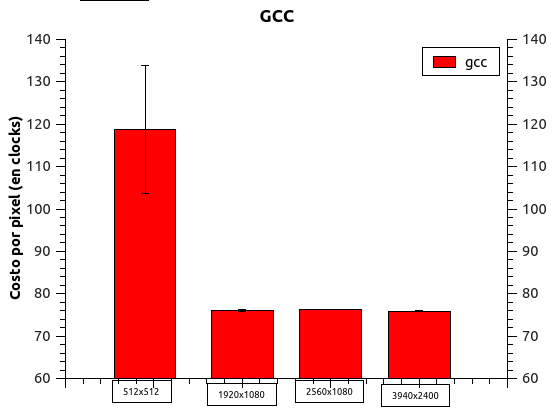
\includegraphics[width=\linewidth]{tiemposCompiladores/gcc.png}
  \caption{{\small Medicion de gcc}} 
\endminipage
\end{center}
\end{figure}

\begin{figure}[H]
\begin{center}
\minipage{0.8\textwidth}
  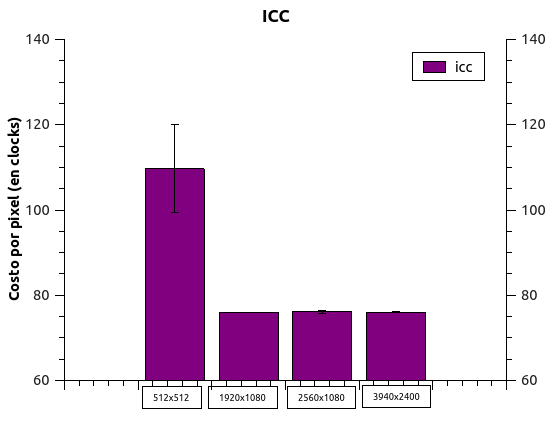
\includegraphics[width=\linewidth]{tiemposCompiladores/icc.png}
  \caption{{\small Medicion de icc}} 
\endminipage
\end{center}
\end{figure}

\begin{figure}[H]
\begin{center}
\minipage{0.8\textwidth}
  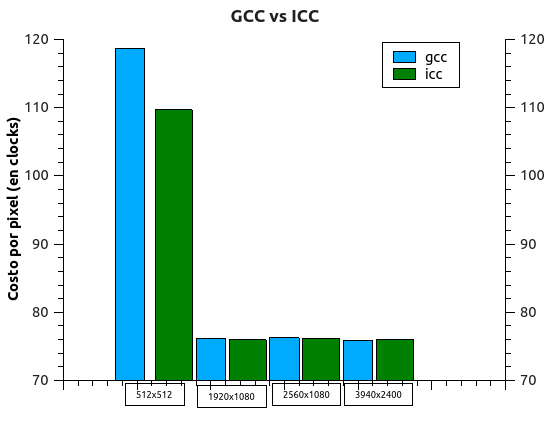
\includegraphics[width=\linewidth]{tiemposCompiladores/gccVsIcc.png}
  \caption{{\small Comparacion entre gcc y icc}} 
\endminipage
\end{center}
\end{figure}

Podemos analizar las siguientes cosas de los resultados obtenidos: \\
Primero, en la imagen mas pequeña, el tiempo de procesamiento por pixel es bastante mayor que en las imagenes mas grandes, en las cuales el tiempo por pixel es casi el mismo. Esto sucede en ambos compiladores. Creemos que esto puede deberse a que hay alguno/algunos procesos en la computadora que no son constantes (es decir, no ocurren cada x cantidad de ciclos) y que influyen en los tiempos. Por eso para imagenes pequeñas se nota su influencia, pero para imagenes grandes no. Tiene sentido entonces, que la desviacion estandar nos de mucho mas alta en la imagen de menor tamaño.\\
Segundo, si bien para la imagen mas pequeña se puede observar que el compilador icc procesa mas rapido, no existe tal diferencia a la hora de procear imagenes mas grandes. Incluso, en la imagen mas grande, es mas rapido (aunque la diferencia es cercana al 1$\%$)
En estas primeras observaciones no tenemos ninguna evidencia que confirme o refute nuestra hipótesis. Vamos a experimentar ahora con ambos compiladores con las opciones de optimización activas.

\subsection{GCC vs ICC con optimización }

Para esta parte del experimento lo que vamos a hacer es activar la opción \textit{-O3} para ambos compiladores. Una vez activada esta opción vamos a realizar devuelta los experimentos para tratar de ver como influye esta opción en el costo temporal de los filtros.Estos experimentos los vamos a realizar con varias imágenes, aplicandoles el filtro Blur con varios valores distintos y comparando los resultados.\\
Las siguientes imágenes detallan estos resultados.\\
Nota: Los valores acá detallados no representan el valor real sino una equivalencia a la hora de graficar. Para obtener el valor real es necesario multiplicar el valor del gráfico por \textit{1.0x106}.\\


\begin{figure}[H]
\begin{center}
\minipage{0.8\textwidth}
  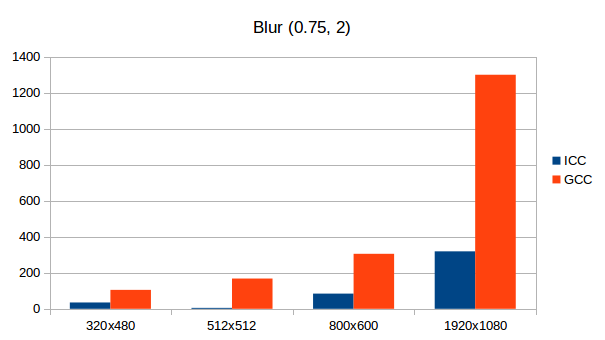
\includegraphics[width=\linewidth]{cachecompiladores/blur0752.png}
  \caption{{\small Blur (0.75, 2)}} 
\endminipage
\end{center}
\end{figure}

\begin{figure}[H]
\begin{center}
\minipage{0.8\textwidth}
  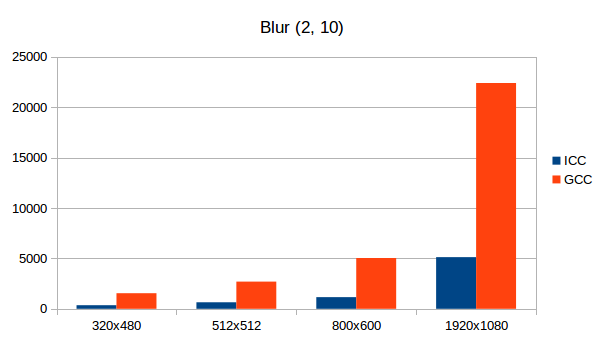
\includegraphics[width=\linewidth]{cachecompiladores/blur210.png}
  \caption{{\small Blur (2, 10)}} 
\endminipage
\end{center}
\end{figure}


\subsection{Conclusion}
Como muestran los graficos anteriores podemos observar una amplia diferencia a favor del ICC y la ventaja no hace más que aumentar a mayor tamaño de imágen y a mayor radio.\\
A estas alturas podemos afirmar que el compilador ICC es mucho mayor que el compilador GCC y así podemos corroborar definitivamente nuestra hipótesis original.\\
A continuacion vamos a realizar varios experimentos más y esta vez no vamos a medir el factor tiempo sino que vamos a evaluar el manejo de la caché por parte de ambos compiladores para ver si esta ventaja se debe a un manejo más eficiente.
Compararemos mas adelante el uso de la cache, pero, a priori, no vemos ninguna ventaja a favor del ICC.
